%---------------------------------------------------------------------
\documentclass[12pt, letterpaper]{article}
\usepackage[utf8]{inputenc}
\usepackage[T1]{fontenc}
\usepackage[spanish,mexico]{babel}
% ajuste de margenes
\usepackage[left=2.5cm,right=2.5cm,top=2.5cm,bottom=2.5cm]{geometry}
\linespread{1}
\pagestyle{headings}
\setlength{\parindent}{0pt} % Elimina auto identacion en parrafos
%---------------------------------------------------------------------
%CONFIG DE TEOREMA
\usepackage{tikz,lipsum,lmodern}
\usepackage[most]{tcolorbox}
\newtcbtheorem[auto counter,number within=section]{theo}%
  {Theorem}{fonttitle=\bfseries\upshape, fontupper=\slshape,
     arc=0mm, colback=blue!5!white,colframe=blue!75!black}{theorem}
%---------------------------------------------------------------------
\usepackage{enumitem}% enumerates
\usepackage{verbatim} 
\usepackage{minted}%code listing
\usepackage{svg}
\usepackage{caption} %imgs dentro de enumerciones
\usepackage{amssymb}
\usepackage{amsmath}
\usepackage{tikz}
\usetikzlibrary{calc, arrows}
%\usepackage{xcolor} %{\color{blue} texto}
\usepackage{xcolor}%[dvipsnames]
\definecolor{mygreen}{RGB}{29, 131, 72}
\usepackage{mathtools}
\usepackage{epigraph}%epígrafe \epigraph{text}{\textit{Richard Courant}}
\usepackage{dirtytalk}%\say{}
\usepackage{graphicx}%imagenes en texto
\usepackage{hyperref}% para hipervinculos
\hypersetup{
    colorlinks=true,
    linkcolor=blue,
    filecolor= {35, 155, 86},      
    urlcolor=mygreen,
    pdftitle={Alexis Tercero},
    pdfpagemode=FullScreen,
    }
%---------------------------------------------------------------------
\author{Alexis Tercero: alexistercero55@gamil.com}
% elimina las ojas blancas extras despues del titulo y tabla de contenidos
\let\cleardoublepage=\clearpage 
%---------------------------------------------------------------------
%---------------------------------------------------------------------
%---------------------------------------------------------------------
\begin{document}
%---------------titulo-----------------------------------------------

%------------------------------------------------------------
%------------------------------------------------------------

\rule{\textwidth}{1pt}
\begin{center} %indicador de seccion/ introducion
    \bfseries Tarea 2 \\ Alexis Uriel Tercero López\\Modelado jerárquico de objetos 3D con OpenGL
\end{center}
\rule{\textwidth}{1pt}

\begin{itemize}
    \item Sistema operativo: Windows 10
    \item Compilar gcc tarea2.c -lfreeglut -lopengl32 -lglu32
\end{itemize}

\section{Descripción del modelo}
Se ha modelado una pirámide de un estilo similar a la maqueta que se monto en el Zócalo de la CDMX
para la conmemoracion de la caida de Tenochtitlan.

\subsection{Primitivas usadas}
\begin{itemize}
    \item Cubos (\texttt{glutSolidCube}).
    \item Esferas (\texttt{glutSolidSphere}).
    \item Planos.
    \item Cilindro (\texttt{gluCylinder}).
\end{itemize}

\section{Código fuente}
\begin{minted}
[
frame=lines,
framesep=2mm,
baselinestretch=1.2,
fontsize=\scriptsize,
linenos %numeracion de lineas
]
{c}
/*  Alexis Tercero: https://github.com/AlexisTercero55
                    alexistercero55@gmail.com
    build command: gcc tarea2.c -lfreeglut -lopengl32 -lglu32
    build task@\.vscode\task.json : ctrl + shift + b
    ------------------------------------------------------------
                            TAREA #2
            Modelado jerárquico de objetos 3D con OpenGL
    ------------------------------------------------------------
    Descripción
    Las y los estudiantes desarrollarán un programa en lenguaje C o C++ que inicializará
    una ventana de GLUT/FreeGLUT donde se desplegará un objeto o escena 3D básica de
    su preferencia hecha con modelado jerárquico, utilizando al menos tres primitivas
    geométricas de GLUT/FreeGLUT y transformaciones geométricas de OpenGL.
    Mientras se ejecuta el programa, el usuario podrá presionar teclas en su teclado,
    esperando ver una respuesta en el programa de acuerdo con la siguiente tabla.

    Tecla   Respuesta esperada
    W / w   Trasladar el modelo 0.1 unidades sobre el eje y.
    S / s   Trasladar el modelo −0.1 unidades sobre el eje y.
    A / a   Trasladar el modelo −0.1 unidades sobre el eje x.
    D / d   Trasladar el modelo 0.1 unidades sobre el eje x.
    I / i   Rotar el modelo −5° sobre sobre el eje x.
    K / k   Rotar el modelo 5° sobre sobre el eje x.
    J / j   Rotar el modelo 5° sobre sobre el eje y
    L / l   Rotar el modelo −5° sobre sobre el eje y
    +       Escalar el modelo 0.1 unidades en todos los ejes.
    -       Escalar el modelo −0.1 unidades en todos los ejes.
    ESC     Termina el programa

    Otra    A su criterio. Pueden no hacer nada.
    Z / z   Traslacion 0.1 en Z.
    X / x   Traslacion -0.1 en Z.
    B / b   Rotacion 5° sobre eje Z.
    N / n   Rotacion -5° sobre eje Z.
    P / p   Cambio de proyeccion.
    M / m   Cambio de modo de dibujo.
*/
#include <stdlib.h>
#include <GL/glut.h>    //-lfreeglut
#include <GL/glu.h>     //-lglu32
#include <GL/gl.h>      //-lopengl32
#include <math.h>

/*PROTOTIPOS*/
void configVentanaGlut(void);
void dibujar(void);
void teclado (unsigned char key, int x, int y);
void camara(void);
void config_OGL();
void redimensionar (int ancho, int alto);
void transformacionesGUI(void);

//Modelo
void escaleras(GLdouble r,GLint h);
void piramide(void);
void ejes(void);
void cilindroSolidWireframeGlut(GLdouble base, GLdouble top, GLdouble height,
 	                            GLint slices, GLint stacks);
void plano_xy(GLfloat L);
void cuboSolidWireframeGlut(GLdouble size);
void esferaSolidWireframeGlut(GLdouble radius, GLint slices, GLint stacks);

//Variables de traslación en X y Y.
GLfloat tx = 0;
GLfloat ty = 0;
GLfloat tz = 0;
//Variables de rotación en X y Y.
GLfloat rx = 0;
GLfloat ry = 0;
GLfloat rz = 0;
//Variable de escala en todos los ejes.
GLfloat es = 1;
//INDICADORES DE ESTADO
GLboolean WIREFRAME_STATE = GL_FALSE;
GLboolean proy_orto = GL_FALSE;

int main(int argc, char** argv) 
{
    glutInit(&argc, argv);
    configVentanaGlut();
    config_OGL();
    glutMainLoop();
    return 0;
}

void transformacionesGUI(void)
{
    glRotatef(rx, 1, 0, 0);
    glRotatef(ry, 0, 1, 0);
    glRotatef(rz, 0, 0, 1);
    glScalef(es, es, es);
}

void cuboSolidWireframeGlut(GLdouble size)
{
    WIREFRAME_STATE ? glutWireCube(size) : glutSolidCube(size);
}

void escaleras(GLdouble r,GLint pisos)
{
    GLfloat p = 2.4; //posicion inicial de escalon
    GLfloat L = 0.2;
    GLint ne = pisos*5;//numero de escalones

    for(int i=0; i < ne; ++i)
    {
        glPushMatrix();//simulacion de coordenadas locales
            glTranslated(p,-p,i*L);
            glRotatef(45,0,0,1);
            glScalef(r,0.4,L);
            glColor3f(0.44,0.34,0.56);//morado
            cuboSolidWireframeGlut(1);
        glPopMatrix();
        p -= 0.1;
        r -= 0.2;
    }
    glColor3f(1,1,1);//blanco
}

void piramide(void)
{
    GLint h = 1;//altura de piso de piramide
    GLfloat R = 4.5;//radio de base
    GLfloat r = 4;//radio de piso, longitud = 2r

    escaleras(r,3*h);

    //piso 1
    glColor3f(0.21,0.94,0.27);//verde
    cilindroSolidWireframeGlut(R, r, h, 4, 1);//cuerpo
    glPushMatrix();//simulacion de coordenadas locales
        glTranslated(0,0,h);
        glRotatef(45, 0, 0, 1);
        plano_xy(sqrt(2)*r);//piso
    glPopMatrix();

    //piso2
    R = R - 1;
    r = r - 1;
    glPushMatrix();//simulacion de coordenadas locales
        glTranslated(0,0,h);
        glColor3f(0.28,0.94,0.92);//azul
        cilindroSolidWireframeGlut(R, r, h, 4, 1);//pisos de la piramide
        glPushMatrix();//simulacion de coordenadas locales
            glTranslated(0,0,h);
            glRotatef(45, 0, 0, 1);
            plano_xy(sqrt(2)*r);//piso
        glPopMatrix();
    glPopMatrix();
        
    //piso 3
    R = R - 1;
    r = r - 1;
    glPushMatrix();//simulacion de coordenadas locales
        glTranslated(0,0,2*h);
        glColor3f(1,0,0.5);//rosa
        cilindroSolidWireframeGlut(R, r, h, 4, 1);//pisos de la piramide
        glPushMatrix();//simulacion de coordenadas locales
            glTranslated(0,0,h);
            glRotatef(45, 0, 0, 1);
            plano_xy(sqrt(2)*r);//piso
        glPopMatrix();
    glPopMatrix();

    r = r - 1;

    //cima de la piramide
    glPushMatrix();//simulacion de coordenadas locales
        glTranslated(0,0,4*h);
        glColor3f(0.44,0.34,0.56);//moradow
        esferaSolidWireframeGlut(r, 5, 2);
    glPopMatrix();
    
    glColor3f(1,1,1);//blanco
}

void ejes(void) 
{
    glBegin(GL_LINES);
        //Eje X
        glColor3f(0,1,0);//verde
        glVertex3f(-10, 0, 0);
        glVertex3f(10, 0, 0);
        //Eje Y
        glColor3f(1,0,0);//rojo
        glVertex3f(0, -10, 0);
        glVertex3f(0, 10, 0);
        //Eje Z
        glColor3f(0,0,1);//azul
        glVertex3f(0, 0, -10);
        glVertex3f(0, 0, 10);
    glEnd();
    glColor3f(1,1,1);
}

void cilindroSolidWireframeGlut(GLdouble base, GLdouble top, GLdouble height,
 	                            GLint slices, GLint stacks)
{
    //paso 1
    GLUquadricObj *quad = gluNewQuadric();
    //paso 1.1
    gluQuadricNormals(quad,GLU_SMOOTH);
    //paso 2
    WIREFRAME_STATE ? gluQuadricDrawStyle(quad,GLU_LINE) : 
                      gluQuadricDrawStyle(quad,GLU_FILL);
    //paso 3
    gluCylinder(quad, base, top, height, slices, stacks);
}

void esferaSolidWireframeGlut(GLdouble radius, GLint slices, GLint stacks)
{
    WIREFRAME_STATE ?  glutWireSphere( radius,  slices,  stacks) : 
                       glutSolidSphere( radius,  slices,  stacks);
}

void plano_xy(GLfloat L) //L : longitud de cada lado
{
    GLenum m; 
    WIREFRAME_STATE ? glBegin(GL_LINE_LOOP) : glBegin(GL_QUADS);
        glVertex3f(-L/2, L/2, 0);
        glVertex3f(L/2, L/2, 0);
        glVertex3f(L/2, -L/2, 0);
        glVertex3f(-L/2, -L/2, 0);
    glEnd();
}

void redimensionar (int ancho, int alto) 
{
    if (alto == 0) alto = 1;
    int lado = ancho < alto ? ancho : alto;
    glViewport((ancho - lado) / 2, (alto - lado) / 2, lado, lado);
    camara();
}

void config_OGL()
{
   camara();
   //habilitar uso de buffers
   glEnable(GL_LIGHTING);//ILUMINACION EN GENERAL
   glEnable(GL_LIGHT0);//LUS ESPECIFICA
   glEnable(GL_DEPTH_TEST);//ACTIVA EL USO DELBUFFER DE PROFUNDIDAD.
   glClearColor(0,0,0,1);//color de fondo.
   glEnable(GL_COLOR_MATERIAL);
}

void camara(void)
{
    /*FUNCION QUE CONFIGURA LA PERSPECTIVA DE LA ESCENA
      Y EL VOLUMEN DE RECORTE DE RENDERIZADO*/
    float ancho = GLUT_WINDOW_WIDTH;
    float alto = GLUT_WINDOW_HEIGHT;
    glMatrixMode(GL_PROJECTION);//indica CAMBIOS EN LA MATIZ DE PROYECCION
    glLoadIdentity();

    //SE INDICA EL TIPO DE PROYECCION
    if (proy_orto){ //ORTOGRAFICA
        glOrtho(-5, 5, -5, 5, -5, 5);
    }
    else{ //EN PERSPECTIVA
        gluPerspective(45, ancho/alto, 0.1, 1000);
        gluLookAt(10, -10, 6, 0, 0, 0, 0, 0, 1);
    }

    glMatrixMode(GL_MODELVIEW);//SE REGISTRAN LOS NUEVOS CAMBIOS
    glLoadIdentity();// LIMPIAR EL RESULTADOS DE LA ESCENA
}

void configVentanaGlut(void)
{
    //configuracion de pantalla
    /*SE RESERVA MEMORIA PARA LOS BUFFERS DE COLOR, DOBLE Y DE PROFUNDIDAD*/
    glutInitDisplayMode(GLUT_RGBA | GLUT_DOUBLE | GLUT_DEPTH);
    glutInitWindowSize(800, 600);
    glutInitWindowPosition(0,0);
    glutCreateWindow("Alexis Tercero 9/19/21 Tarea 3 : Modelado jerarquico de objetos 3D con OpenGL");
    //registro y ejecuccion de procesos
    glutDisplayFunc(dibujar);//LO QUE SE RENDERIZA
    glutKeyboardFunc(teclado);//INTERACTIVIDAD : REAL-TIME 3D
    glutReshapeFunc(redimensionar);//USER EXPERIENCE
}

void dibujar(void) 
{
    //LIMPIAR BUFFERS DE COLOR Y DE PROFUNDIDAD.
    glClear(GL_COLOR_BUFFER_BIT | GL_DEPTH_BUFFER_BIT);

    glPushMatrix();
        glTranslatef(tx, ty, tz);
        transformacionesGUI();
        piramide();
        ejes();
    glPopMatrix();
    
    ejes();
    glutSwapBuffers(); //hacer cambio de buffers (HABILITAR BUFFERDOBLE POR FREEGLUT)
}

void teclado (unsigned char key, int x, int y) 
{
    switch (key) 
    {
        case 27: //scape in ASCII
            exit(0); break;

        case 'p': case 'P'://CAMBIAR ENTRE PERSPECTIVAS DE LA ESCENA
            proy_orto = !proy_orto;
            camara();  break;

        case 'M': case 'm'://CAMBIAR ENTRE MODO SOLIDO Y WIREFRAME
            WIREFRAME_STATE = !WIREFRAME_STATE; break;
        //TRASLACIÓN
        case 'W': case 'w': ty += 0.1; break;
        case 'S': case 's': ty -= 0.1; break;
        case 'A': case 'a': tx -= 0.1; break;
        case 'D': case 'd': tx += 0.1; break;
        case 'Z': case 'z': tz += 0.1; break;
        case 'X': case 'x': tz -= 0.1; break;
        //ROTACIÓN
        case 'I': case 'i': rx += 5; break;
        case 'K': case 'k': rx -= 5; break;
        case 'J': case 'j': ry += 5; break;
        case 'L': case 'l': ry -= 5; break;
        case 'B': case 'b': rz += 5; break;
        case 'N': case 'n': rz -= 5; break;
        //ESCALA
        case '+': es += 0.1; break;
        case '-': es -= 0.1; break;
        default: break;
    }
    //INDICAR AL O.S. QUE DIBUJE YA
    glutPostRedisplay(); //optimizacion de recursos
}
\end{minted}
%-------------------------------------------------------
\newpage
\section{Salida del programa: capturas de pantalla}
\begin{figure}[h!]
    \centering
    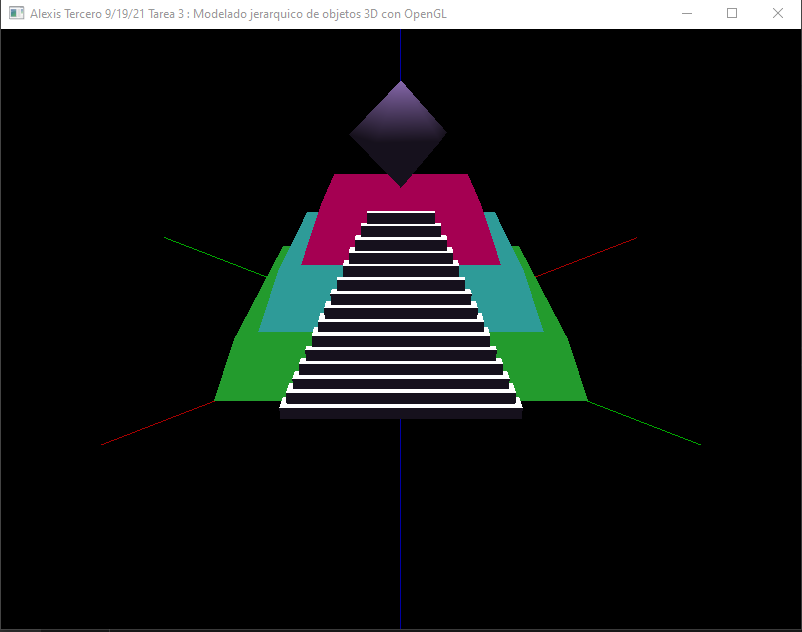
\includegraphics[scale=0.4]{1.png}
    \caption{Modelo en posición inicial.}
\end{figure}

\begin{figure}[h!]
    \centering
    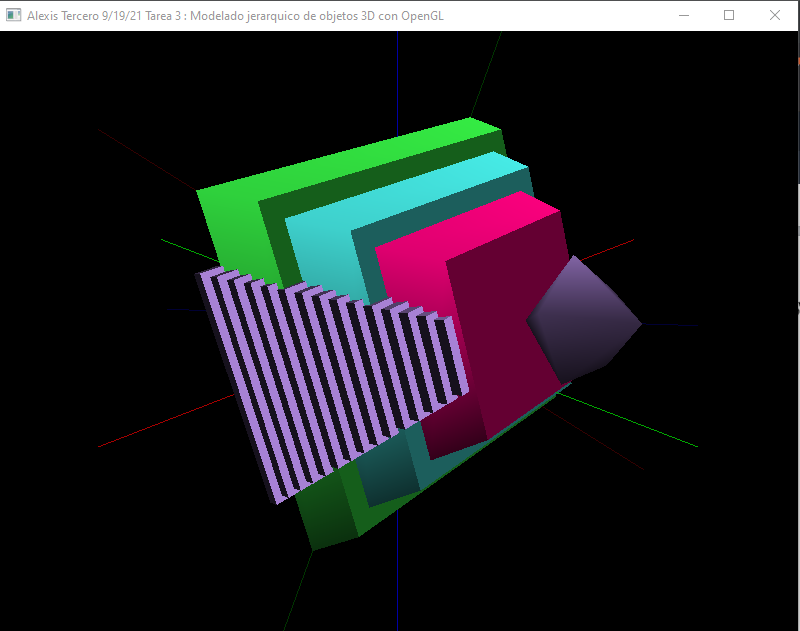
\includegraphics[scale=0.4]{2.png}
    \caption{Ración en z -45°, traslado -1 en y 1 en x, 1en z, rotación 55° en y por ultimo rotación -5° en x}
\end{figure}
\newpage
%-------------------------------------------------------
\section{Extras}



\subsection{GitHub}
Se invita al lector a visitar el repositorio remoto 
\href{https://github.com/AlexisTercero55/practicasOpenGL}{AlexisTercero55/practicasOpenGL}
creado con el fin de registrar el aprendizaje a lo largo del curso. En el repositorio usted podrá encontrar notas del curso, practicas y tareas a través de la rama master.\vspace{2ex}

URL: \url{https://github.com/AlexisTercero55/practicasOpenGL}




%\hspace{1ex} \vspace{1ex} \begin{pmatrix}\end{pmatrix} \mathbb{R} \vrule ¿?\langle  \rangle \Big(\Big) \left|  \right|
%Wolfram command for jacobian jacobian matrix () with respect to (x_1,x_2,x_3)
\end{document}